
\section{Compiler Infrastructure}

Compilers are programming tools responsible for translating programs in a given source language to a lower-level target language.
This compilation process must preserve the program semantics.
Moreover, compilers are also expected to produce a good quality representation of the program in the target language, optimising for a given objective function.
An important objective function is code size, i.e., the optimisation goal is to produce a representation of the program as small as possible.

%Compilers must preserve the program semantics.

In order to manage their complexity, compilers are usually designed in a highly modular manner, where they are organised as a series of phases that sequentially analyse and transform the program being compiled.
In their simplest form, compilers are usually organised in \textit{three-phases}, as shown in Figure~\ref{fig:3-phase-compiler}: frontend, optimiser, and backend.
The frontend is responsible for parsing, validating and diagnosing errors in the source code.
This parsed source code is then translated into an intermediate representation, which is the LLVM IR in this case.
The optimiser is responsible for doing a broad variety of transformations, that are usually independent of language and target machine, to improve the code's performance.
The backend, also known as the code generator, then translates the code from the intermediate representation onto the target instruction set.
It is common for the backend to also perform some low-level optimisations that take advantage of unusual features of the supported architecture.
%Common parts of a compiler backend include instruction selection, register allocation, and instruction scheduling.

\begin{figure}[h]
  \centering
  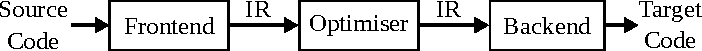
\includegraphics[scale=0.9]{src/background/figs/3-phase-compiler.pdf}
  \caption{Overview of the three-phase compiler infrastructure.}
  \label{fig:3-phase-compiler}
\end{figure}

%The front end parses source code, checking it for errors, and builds a language-specific Abstract Syntax Tree (AST) to represent the input code. The AST is optionally converted to a new representation for optimization, and the optimizer and back end are run on the code.
%The optimizer is responsible for doing a broad variety of transformations to try to improve the code's running time, such as eliminating redundant computations, and is usually more or less independent of language and target.


\begin{figure}[h]
  \centering
  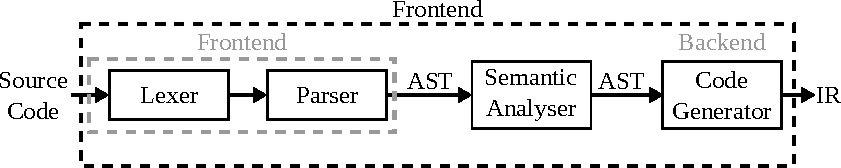
\includegraphics[scale=0.9]{src/background/figs/compiler-frontend.pdf}
  \caption{Overview of the three-phase compiler infrastructure.}
  \label{fig:compiler-frontend}
\end{figure}

\begin{figure}[h]
  \centering
  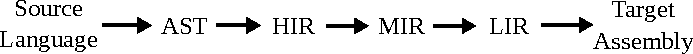
\includegraphics[scale=0.9]{src/background/figs/ir-lowering-sequence.pdf}
  \caption{Overview of the three-phase compiler infrastructure.}
  \label{fig:ir-lowering-sequence}
\end{figure}

\subsection{Link-Time Optimisations}
%% benefits of LTO
%% challenges with LTO
%% mention partial LTO, such as ThinLTO

\begin{figure}[h]
  \centering
  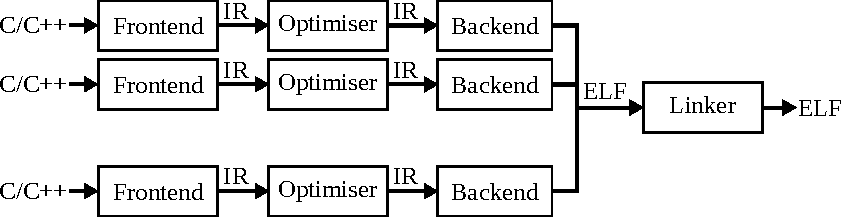
\includegraphics[scale=0.85]{src/background/figs/full-pipeline.pdf}
  \caption{Overview of the three-phase compiler infrastructure.}
  \label{fig:ir-lowering-sequence}
\end{figure}

\begin{figure}[h]
  \centering
  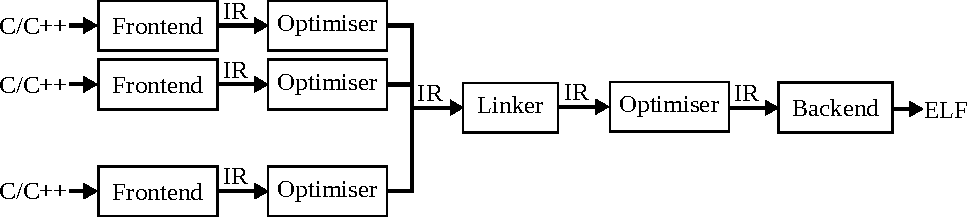
\includegraphics[scale=0.85]{src/background/figs/full-pipeline-LTO.pdf}
  \caption{Overview of the three-phase compiler infrastructure.}
  \label{fig:ir-lowering-sequence}
\end{figure}
